\documentclass[8pt]{article}
\title {Estimating the number of COVID-19 victims by combining the
general logistic model with the pCN Monte Carlo sampling}

\usepackage{graphicx}
\usepackage{verbatim}
\usepackage{amsthm}
\usepackage{amssymb}
\usepackage{amsmath}
\newtheorem{deff}{Definition}
\usepackage{graphicx}
\usepackage{subcaption}
\usepackage[font=small,labelfont=bf]{caption}


\newcommand{\norm}[1]{\left\lVert#1\right\rVert}
%\newtheorem{theorem}{Proposition}
\newtheorem{definition}{Definition}
\newtheorem{Proposition}{Proposition}

\begin{document}
\maketitle
\section{Introduction}
A simply effective way to quantify an epidemic
impact, is given by counting the number of deaths.
We are interested in using that number
to better understand in which scenario we are likely to fall 
in the short and long term future.


To model the number of victims in time, we choose
a generalized logistic map $X^P(t)$ governed by an unknown parameter 
$P \in \mathbb{R}^3$. Then, by using the Preconditioned Crank-Nicolson
MCMC method on the available data,
we establish what are the various possibilities
for the  
values of $P$. Finally, by using the just learned values,
running the model with them gives the various possibilities
for the number of victims in the upcoming future.


Concretely speaking, we work with the most afflicted European Countries
(Italy, Spain, Germany, France, UK). Our final
goal is to answer to the following question:
under the assumptions above,
\textbf{
how many $n$ weeks of data do we need if we want to produce a prediction 
lasting for (at least) the next $m$ weeks}?


We conclude by showing encouraging numerical results, suggesting that
the chosen way might be good, but there are still possibilities of improvement.

\section {The generalized logistic model}
We choose to model the number of deaths in time with a
generalized logistic function. 
Recall that these maps are all
$S$-shaped curves, intuitively seen as an exponential start,
then slowed down until reaching an horizontal equilibrium. 


We do not provide any deep epidemiological explanation for such a choice,
except that we expect a similar qualitative behavior for the phenomenon
under analysis: the number of deaths is supposed to be higher at the beginning,
reaching then a saturation point as long as the health system becomes
capable of managing the emergency.


Of course, we are not new in proposing these maps: in the literature,
there is a wide range of successful applications in similar fields (REF).


Our general logistic map is given by the following 1-dimension ODE:
\begin{equation}
	X'(t) = \frac{q}{v} X(t) 
	\left ( 1 - \left( \frac{X(t)}{Q} \right)^{v}\right )
\end{equation}
with closed form solution:
\begin{equation}
	X(t) = \frac{Q} { (1 + A \exp[-q t])^{\frac{1}{v}}}
\end{equation}

for three (in theory) \emph{stricly positivive} real parameters, 
$P = \{ q, Q, v\}$ and initial time zero condition $X_0$
(we write $X(t) = X^P(t) = X^P_{X_0}(t)$ to stress this dependence).
The letter $A$ abbreviates 
$A = -1 + \left ( \frac{Q} { X_0} \right )^{v}$.


Due to the limit $\lim_{t \to \infty} X(t) = Q$, 
we interpret $Q$ as
the maximum value reached asymptotically, sometimes
referred as the \emph{carrying capacity} in the literature.


The parameter $v$ is related to the symmetry of the curve.
Its limit for $v \to 0^+$ produces the \emph{Gompertz} model,
while the case $v = 1$ the \emph{simple} logistic map.


The simple logistic model suggest an interpretation for the quantity
$q$, too. In such a case the equation would just be
\begin{equation}
	X'(t) = q X(t) 
	\left ( 1 - \left( \frac{X(t)}{Q} \right)\right )
\end{equation}
For very small time the value $X(t)$ is surely far lower than
$Q$ (otherwise the system would already be in equilibrium), therefore
we would have $X'(t) \approx q X(t)$, giving so
$q$ as the rate of the starting exponential growth.


\section{The bayesian approach}
Let $X^P_{X_0}(t)$ be always the generalized logistic model above,
depending on
parameters $P$ and with $X_0$ time zero condition.
When using the model in practice, we can only observe a
limited amount of points coming from its ODE trajectory, 
which are furthermore perturbed by a noise due to measurement
errors.
Let's fix $T+1$ times $\{t_i\}_{i = 0,\dots, T}$.
In our experiments, $T$ is generally between 7 and 21 days.

\begin{definition}
	The \emph{observed vector} $\textbf{y} \in \mathbb{R}^{T+1}$
	is the random variable defined componentwise as:

\begin{equation}
	y_i(\omega) = X^P_{X_0} (t_i) + \eta_i(\omega)
\end{equation}
where $\eta_i \sim \mathcal{N}(0, \sigma^2_i)$.
\footnote{Sometimes by an abuse of notation 
we use the symbol $\eta_i$ to indicate its density function too,
so writing $\eta_i(x)$ for $x \in \mathbb{R}$ refers to that.}
\end{definition}


In other words, $y$ represents the actual measurements on which we
assume the influence of random errors. An important assumption that
we make, lies in the belief that the errors follow the
Gaussian structure above. In principle, many other possibilities
can be chosen.
In practice, the choice above is pretty standard and 
seems to work reasonabily well.
We consider the measurements
to be "reliable up to a $10\%$ of error", in the sense that
the "true" value at time $i$ is supposed to be likely in the interval
$y_i \pm \frac{y_i}{10}$.
Recalling that
$\eta_i \sim N(0, \sigma_i^2) \implies 
\mathbb{P}[ - 2 \sigma_i \leq \eta_i \leq 2 \sigma_i] \geq 95\%$, choosing
then the standard deviation
$\sigma_i \doteq \frac{y_i}{20}$ gives an error on $y_i$ as desired.


Intuitively speaking, fitting the model means to estimate
the unknown $P \in \mathbb{R}^3$ \emph{given} the observation of $\textbf{y}$.
If we interpret $P$ as a random variable, it means that 
the unknown quantity is given by the conditioned
probability $\mathbb{P}[P | y]$.


We start by choosing a \emph{prior} probability measure $\mathbb{P}[P]$ on 
$\mathbb{R}^3$, representing our blind guess about 
$P$ \emph{independently} of the 
observations $\textbf{y}$. In practice this is sometimes an hard guess
which can strongly influence the results.
We will carefully describe our choice in a dedicated section.


If, as just pointed out, we aim at understanding 
$\mathbb{P}[P | \textbf{y}]$, then the classical Bayes's law
$\mathbb{P}[P | \textbf{y}] \propto
	\mathbb{P}[\textbf{y} | P] \times \mathbb{P}[P]$
allows to find it multiplying the the prior  
by an hypothetical conditioned law $\mathbb{P}[\textbf{y} | P]$: this
is where the notion of likelihood comes into play.


\begin{definition}
For every fixed choice of the parameters $P$, the likelihood functions
for the observation of $\textbf{y}$, given $P$, is defined to be:
	\begin{equation}
	\mathcal{L}(\textbf{y}|P) \doteq 
		\frac{(2 \pi)^{- \frac{T}{2}}}
		{\sigma_0\cdots\sigma_{T}}
		\exp \left( -\frac{1}{2} 
		\sum_{i=0}^{T} 
		\frac{(y_i - X_{X_0}^P(t_i))^2}
		{\sigma_i^2}
		\right )
	\end{equation}
\end{definition}


By \emph{interpreting} the likelihood as an effective probability
conditioning, writing informally 
"$\mathbb{P}[\textbf{y}|P] = \mathcal{L}(\textbf{y}|P)$",
not only 
the formula is explained when looking at the noise
distribution $\eta(\textbf{y} - X^P)$, but the 
fitting problem has now a clean solution:

\begin{definition}
	The (Bayesian)
	answer to the problem "Finding the probability density of
	the parameters $P$ given the observations $\textbf{y}$"
	is given by the \emph{posterior}
	distribution on $\mathbb{R}^{3}$ defined by:
	\begin{equation}
		\mu(dx) \propto \mathcal{L}(\textbf{y} | x) \rho(dx)
	\end{equation}
	where $\mathcal{L}$ is the likelihood defined above
	and $\rho$ the prior probability for $P$.
\end{definition}


During every use of the Bayesian rule, we constantly omitted the denominator
relying always on the proportionality "$\propto$". 
This is because such a value is always the probability 
normalization constant,
a number that can be completely ignored in practice thanks to the use
of suitable Monte Carlo techniques.


\subsection{The Preconditioned Crank-Nicolson MCMC}
In the previous section we revised the Bayesian algorithm
as a tool to convert the problem of
estimating the parameter $\mathbb{P} \in \mathbb{R}^3$, to the task
of sampling from the \emph{posterior} probability $\mu$ on $\mathbb{R}^3$.
Its statistical properties convey the information that we need:
for instance, the mode can be read like "the most probably
choice for $P$", its variance can suggest how the uncertainty
is spread, and so on.
In principle one can analyze the posterior analytically,
since it is explicitely given by formula NUMBER.
But usually it is too hard to be done with pen and paper.
Our answer it to use numerical tools: first we
produce a large amount of samples, then we analyze them
statistically.


In order to produce a (single) sample from $\mu$,
we use the so-called Preconditioned
Crank-Nicolson Markov Chain Monte Carlo (pCN).
Briefly speaking, it is a variant of the classic
Gaussian Random Walk, but mainly used for much more complicated cases
where for instance one can \emph{arbitrarily} refine the ODE
trajectory, or when the parameters $P$ belongs to 
an infinite dimensional Banach space, or simply in the context of
PDEs inverse problems.
None of them is our case, since we have just $P \in \mathbb{R}^3$ and
only limited daily available data.


Therefore there is no solid a priori justification for this specific 
Monte Carlo strategy, and one is free to choose another sampling method.
We plan to test and study the various performances, but in another work:
since the final results here are reasonabily fine, we decided
to keep the algorithm for now, leaving potential room for improvement.


The reader is invited in consulting REF for a general exhaustive description
of the pCN MCMC. In our simpler cases, the algorithm follows.


Given two candidate parameters $u, v \in \mathbb{R}^3$
define the acceptance probability:
\begin{equation}
	a(u, v) \doteq \min \{ 1, \frac{ \mathcal{L}(\textbf{y} | v )}
				{\mathcal{L}(\textbf{y} | u)} \}
\end{equation}
and set the \emph{exploratory} parameter $0 < \beta_{pcn} < 1$
(see step 3).
The pCN \emph{requires} the prior distribution $\rho(dx)$
to be a \emph{centered} Gaussian, and used it as proposal step.
This might be, in principle, a strong limitation: more comments about the
prior will fillow in a dedicated section.


To produce a \textbf{single sample} from $\mu$, construct a chain 
$\{ x_i \} _{i \in \mathbb{N} }$ as follows:

\begin{enumerate}
	\item set $x_0 \in \mathbb{R}^n$ \textbf{arbitrarily}. Then, for each
		$k > 0$:
	\item sample a point $R \in \mathbb{R}^3$ 
		from the gaussian prior distribution $\rho(dx)$;

	\item  propose a candidate as 
		$
		\hat{x}_{k} = \sqrt{(1 - \beta^2)} x_{k-1}
			+ \beta R
		$;
	\item	accept it (i.e. set $x_{k} = \hat{x}_{k}$)
		with probability $a(x_{k-1}, \hat{x}_k)$;
	\item (accepted or not) repeat from 2;
\end{enumerate}

To avoid overflow problems, it is suggested to work with
logatithms in the acceptance formula. Define
$N$ to be the integer at which we (always) stop the chain,
so that everytime that we start from a point $x_0$,
the chain produces a sample
$x_N$. The value for $N$ must
be chosen in a way to overtake the known \emph{burning time} issue.
We always set it to be $2^15 > 130000$.


Repeating multiple times the algorithm with \emph{different} starting points
$x_0$,
we collect large amounts of samples, call this number $S$,
where the \emph{correlation} between them, a typical issue when
when using a single traditional Markov Chain,
is hopefully well mitigated. Again, in practice we set this value
as $2^15$, too.


Concerning the conservative parameter $\beta$, it was usually tuned around
$0.001$ or comparable values, chosen in order to produce a chain with
an acceptance rate around $25\%$.


We still have to comment about the choice for the prior $\rho(dx)$ and
the starting points $x_0$. Tt will be done in a section later.

We finally highlight how every chain istance
is independent, therefore the complete sampling prodecure 
is suitable to parallelization
(the user must be warned about the use of a proper seed).


\begin{comment}
\subsection{The k-means algorithm}
TO REWRITE
Once we have a large set of samples from the posterior distribution
(usually more that $5000$ points each of dimension $n$, where 
$x \in \mathbb{R}^n$, i.e. $n$ is the number of parameters to estimate),
we want to actually understand how to use this information.
Therefore we need a strategy to reduce the dimension.
We borrow a simple but strong technique
from the Machine Learning community, called the \emph{k-means} algorithm.


In few words given a cloud of points in $\mathbb{R}^n$, the k-means allows
to divide it in a selected number of \emph{clusters}, call it $k$,
each represented
by a \emph{centroid}. You can think on this algorithm as a multidimensional
way of performing an histogram. Therefore, as for the latter case,
there is no fixed-universal rule for the right amount of centroids.
More regular distributions are likely to be represented well with a few
numbers of them, and for our application we found $k = 5$ to be a fair choice. 
It means than for each observation (dataset) we will have $k$ 
predictions for the same model, each with an associated probability rate.
We underline how this uncertainty comes from the fact of considering
the noise as an intrinsic element of the problem itself.
\end{comment}

\section{Tuning the remaining parameters}

\subsection{Comments on the assumptions and methodology}
We apply the previous theory in order to formulate hypothesis 
for multiple European Countries concerning the future number of
deceased people. We firstly use part of the available data at the beginning
of April to predict the behavior until the mid of May (now known),
verify them, and then
repeating the same methodology for the month of June.
As we briefly said in the introduction, different number of weeks
are taken as input data, in order to observe their predictions' strenght.
A lot of careful points must be checked.


\subsubsection{Why choosing an autonomous ODE}
In the first section we justified the choice of a logistic map by looking
at its S-shaped qualitative behavior, but we didn't comment the
importance of keeping
a curve described by an autonomous ODE.


Since the data in all Countries start around the mid
of February, one might be tempted to use the \emph{entire}
collection (until, e.g. the $10$th of April)
relying on the intuition "more data, more accuracy".


As a first intuitive remark,
recall that the general logistic model is connected to the simple
logistic map ($v = 1$). For the latter one can show that,
when used to model the number of infected,
the map can be reformulated as a $SIS$ compartmental model
where $q$ is also connected to the average number of people's
daily social contacts.
But since lockdown measures have been adopted, this quantity
strongly changed in time. As a consequence of that, although
we have no 100\% rigorous justification,
we prefer \textbf{not} to trust the entire available dataset, but rather
limiting the observations on time period with
\emph{constant} (stronger or weaker) lockdown measures.
Data for each Countries
are given in their sections.


When following this logic, three cases can happen:
\begin{itemize}
	\item[1] the "true" process is actually a general logistic one,
		but it already started \emph{before} we began collecting data;
	\item[2] same as above, but the ODE \emph{still} have
		to start, implying that part of the
		initial data that we read belongs to
		another model/trajectory;
	\item[3] the "true" model is not a general logistic one at all.
\end{itemize}


Of course, we cannot do nothing against $3$, but the final results suggest
that a general logistic model might be a "not-too-bad" choice.
Conversely, by adding some days of delay we can increase the
possibility of not being in 2.
Finally, dealing with the problem number 1,
it is necessary to ensure that the skipped days 
(e.g. including the one skypped in 2)
can actually be "forgotten".
But when choosing an autonomous ODE, this is precisely what
claimed by the semigroup property of its associated flow.
Briefly speaking,
no matter if we start observing a value, say $V_n$, at 
day $n$, or $V_{n+1}$ at day $n+1$: 
the trajectory produced from day $n+1$ (with initial
conditions $V_{n+1}$) is precisely the same as the one
produced by beginning at day $n$ (with initial condition $V_n$).
The two trajectories \emph{are ruled by the same values of $P$},
therefore they infere the same parameter $P$ (i.e. one can safely
start the observations from the day $n+1$).
Of course, one should not abuse this fact:
the more are the observed data belonging the \emph{same}
trajectory, the better the estimation works.
In other words, if one is sure that the ODE started at day $n$,
one should take it as starting day and not $n+1$, in order to
improve the estimator's performance.


\subsection{Choosing the prior distribution}
The goal of this section is to explain in which way we chosen the
prior probability measure $\rho(dx)$.
Since we used the pCN MCMC, it is required to be a centered Gaussian. 
It might represent
a strong limitation, especially if we consider the fact
that all the parameters in the general logistic equation
are supposed to be positive. In order to cincumvent this problem,
we tried with a very straightforward approach (which worked):
we started the chain always with positive values,
and when negative are proposed, we discard them.


Consequently we are technically not considering the full posterior
distribution, but just its part with posisitive values.
Altoight we still have to prove that there are no theoretical
pitfalls, this naive approach seem to work reasonabily well.


\begin{comment}
We did not \emph{impose}
any limitation on the parameter's domain: the chains
were free to explore negative values, too (until the proposals
were not inf or NaN), and we expected the chain to authomatically
reject these values due to possibly worse Likelihood' values.
It was almost always the case, but \emph{very surprisingly}
sometimes negative values for $v$ were preferred!
This is actually not something analytically forbidden, and we kept
such results as an interesting emerging property.


TO DO: STUDYING ANALYTICALLY WHAT HAPPENS WITH NEGATIVE V
\end{comment}


Dealing with the precise structure of the prior distribution and the
chain's starting points, everything is clarified in the following lines.
Remember that the role of $\rho$
is to represent the expected range of the searched values.
For simplicity we define it with an easy covariance form:
\begin{equation}
\begin{pmatrix}
	\sigma_q^2 & 0 & 0 \\
	0 & \sigma_Q^2 & 0 \\
	0 & 0 & \sigma_v^2
\end{pmatrix}
\end{equation}
splitting so the prior into three independent one dimensional Gaussians for
every parameters. Recall that if $X \sim N(0,\sigma^2)$, the classical
quantile property claims 
$\mathbb{P}[-2 \sigma \leq X \leq 2 \sigma] \geq 0.95$.
In the first section we recall how we prefer having $v \in [0,1]$, so by
using the formula above we suggest $\sigma_v = 0.5$.

We remind that $q$ is connected to the simple logistic's
 starting exponential growth, while $Q$ 
relates to the maximum number of possible cases. 
Our idea is simple: as a first move,
we do a rough exponential interpolation on the given dataset. 
Since we always obtained very small exponential powers,
we use this knowledge to set  $\sigma_q = 0.05$
(altought we are using a general logistic map, and not just the
simple logistic model).
Furthermore, the exponential law gives a rough
prediction about the number of the deaths around, say, the $20th$ of May
(i.e. one Month after the datasets); call it $N_e$.
We set $\sigma_Q = \frac{N_e}{2}$, in order to represent the idea
"a good candidate for the true number of deceased people is likely
below the prediction done with the exponential case, being that the
most aggressive accepted model".


Finally, it remains to tune the starting point $x_0 \in \mathbb{R}^3$
for every Markov Chain. Let $D$ be
the least read data from the dataset, i.e. the current
number of deaths.
Not surprisingly, we initialize $x_0$ uniformly randomly in
$[0, 1] \times [D, N_e] \times [0,1]$ coherently which the explanation above.


\section{Numerical results}
We took into account multiple European Countries with the idea of
answering to the following question:
supposing to be in a stable situation capable of avoiding
an exponential explosion of the infection, how many weeks of data do we need
before being able to perform realiable predictions concerning the
number of deceased people?
More precisely, for how many days do last the analysis done by using
$n$ weeks of data?


For each Country, we looked for the day when the lockdown measures
came into play, waited around 15 days (incubation time, so to nullify
the influence of the previous conditions), then we did predictions 
using 1, 2 and 3 weeks of data. They are generally done by using 
the days belonging to the first half of April, with the idea of lasting
at least until the mid of May. Then all the Countries changed their
policy. Therefore the idea is: if we manage to succed in predicting
what happened in May by using the data in April, we can repat the same
strategy concerning the month of June. 


For each Country there is a dedicated section.
Recall that the fitting procedure is done my using a Bayesian algorithm,
producing so a probability measure for the parameters. We split it in
clusters producing multi dimensional histograms, and considered
only the 95\% of its mass, eliminating so the very
unlikely extreme value. We paid attention to
the "worst" case scenario, i.e. the one with the highest number of deaths, 
the "best", and, when possible, the expectation value.


\begin{figure}[h!]
  \centering
  \begin{subfigure}[b]{0.45\linewidth}
  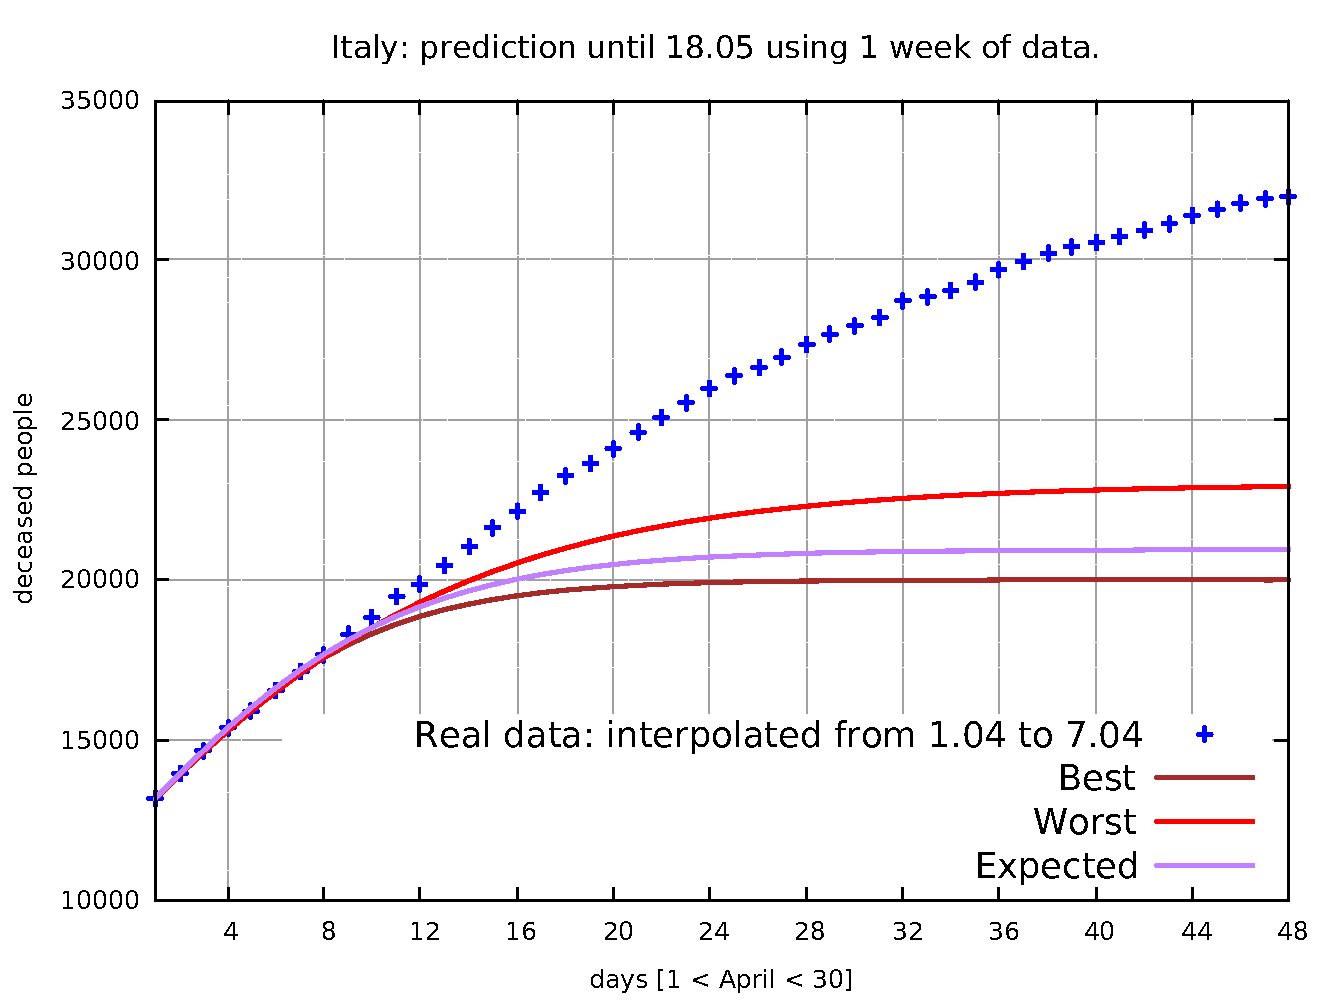
\includegraphics[width=\linewidth]{../simulations_v1/it/1-7/1-7.pdf}
  \end{subfigure}
  \begin{subfigure}[b]{0.45\linewidth}
    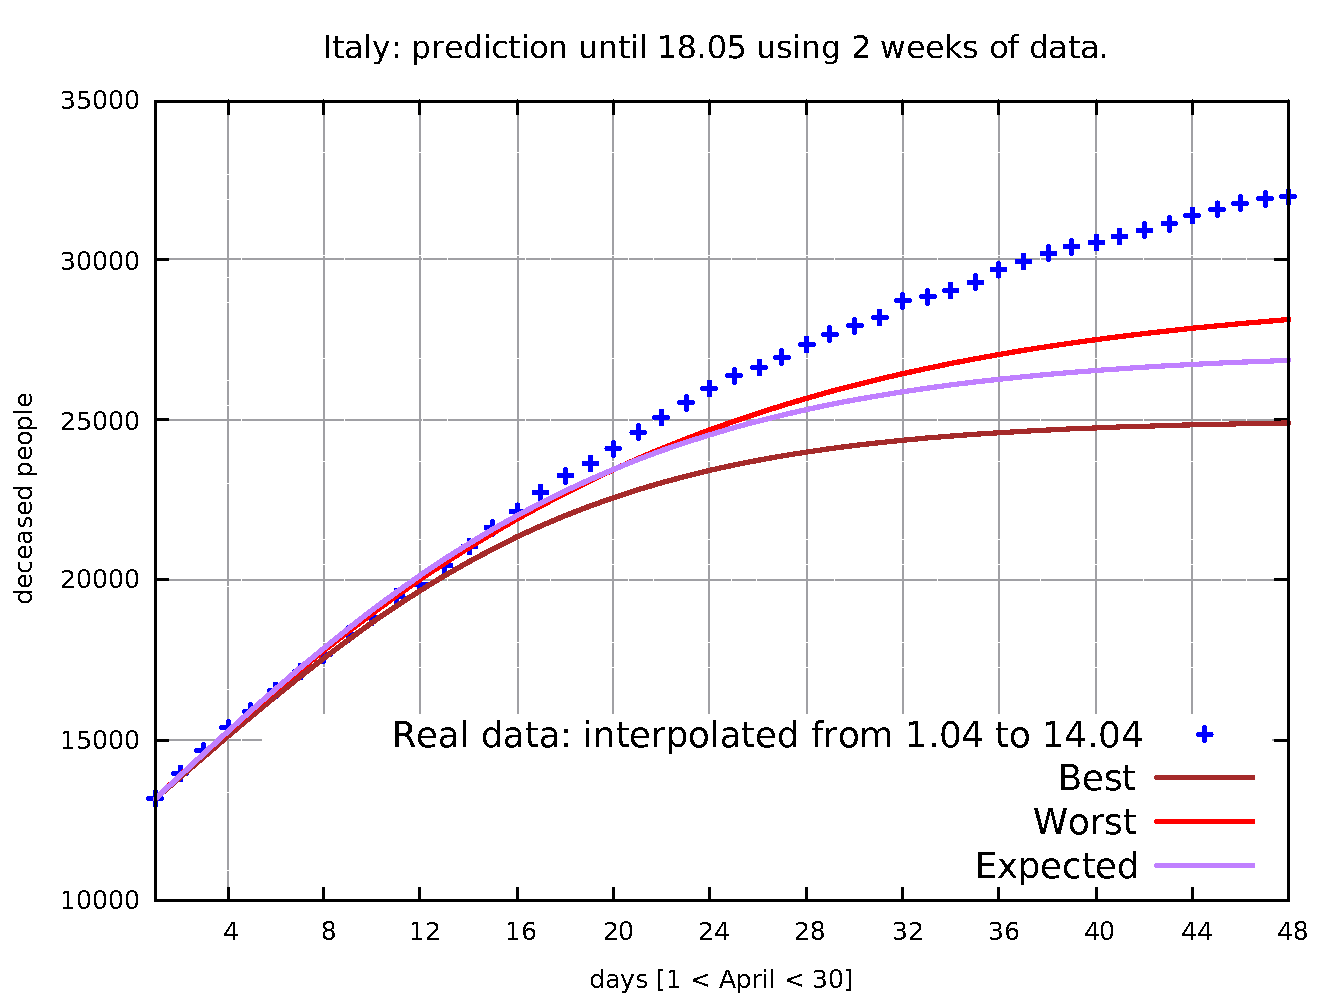
\includegraphics[width=\linewidth]{../simulations_v1/it/1-14/1-14.pdf}
  \end{subfigure}
  \begin{subfigure}[b]{0.45\linewidth}
  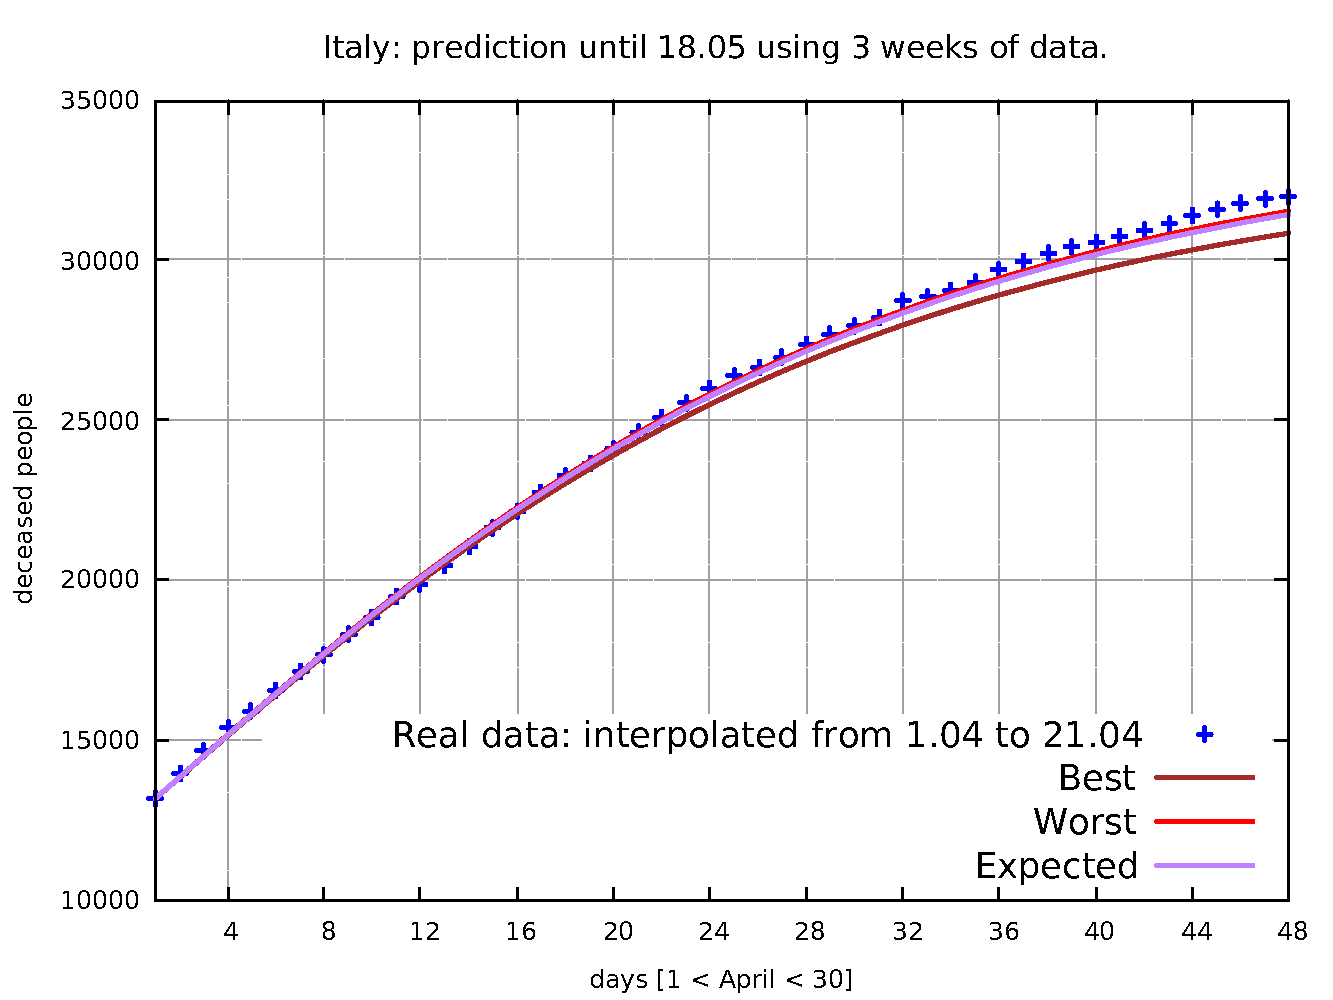
\includegraphics[width=\linewidth]{../simulations_v1/it/1-21/1-21.pdf}
  \end{subfigure}
	\caption{Italy - Lockdown measures were declared on the 15th of March.
                We started gathering the data from the 1st of April.}
\end{figure}


\begin{figure}[h!]
  \centering
  \begin{subfigure}[b]{0.45\linewidth}
  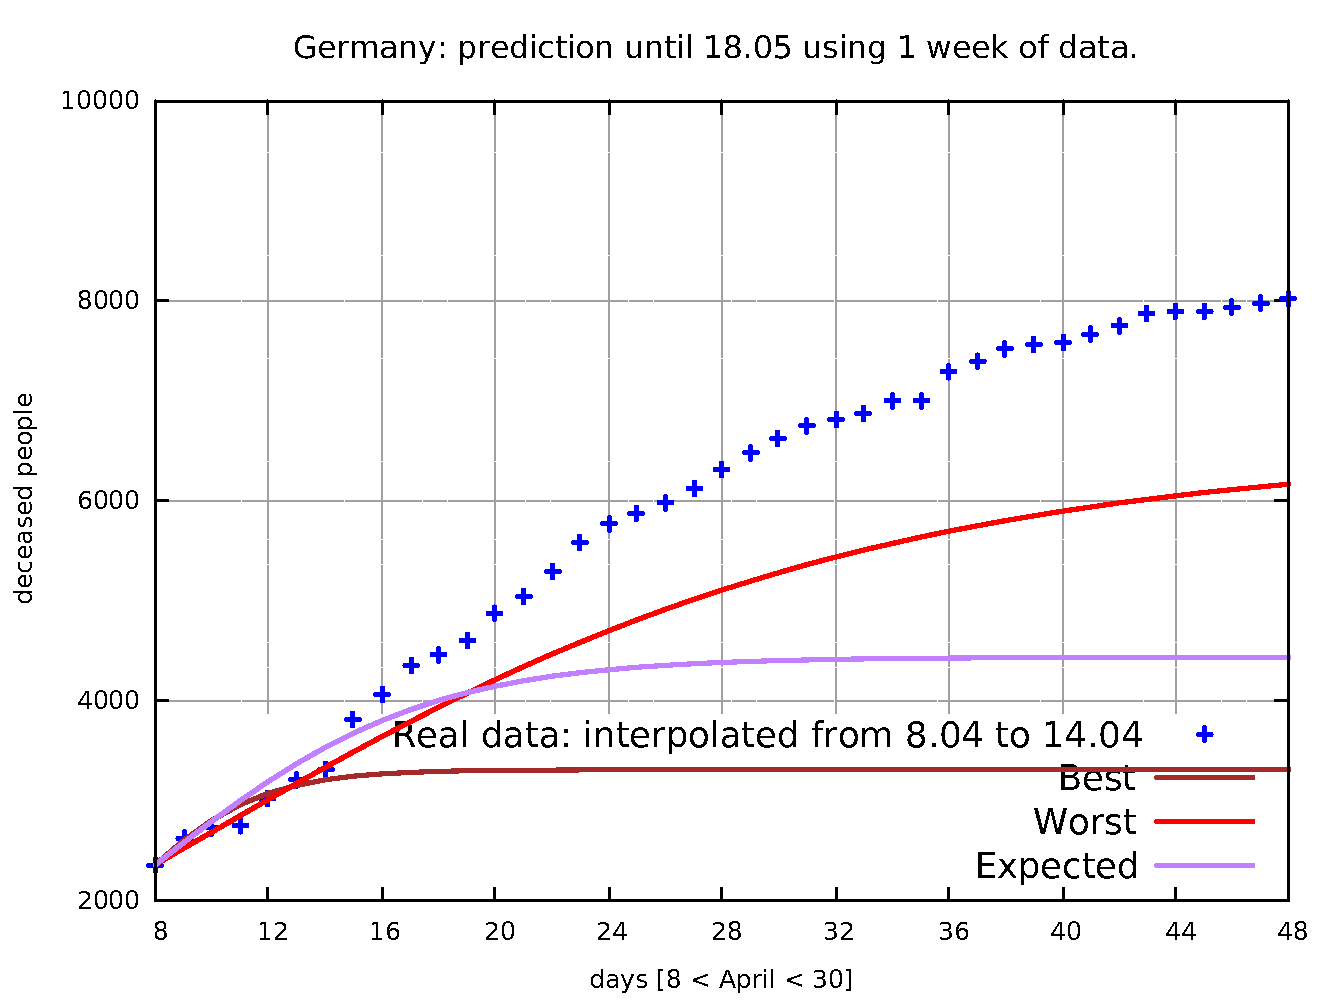
\includegraphics[width=\linewidth]{../simulations_v1/de/8-14/8-14.pdf}
  \end{subfigure}
  \begin{subfigure}[b]{0.45\linewidth}
    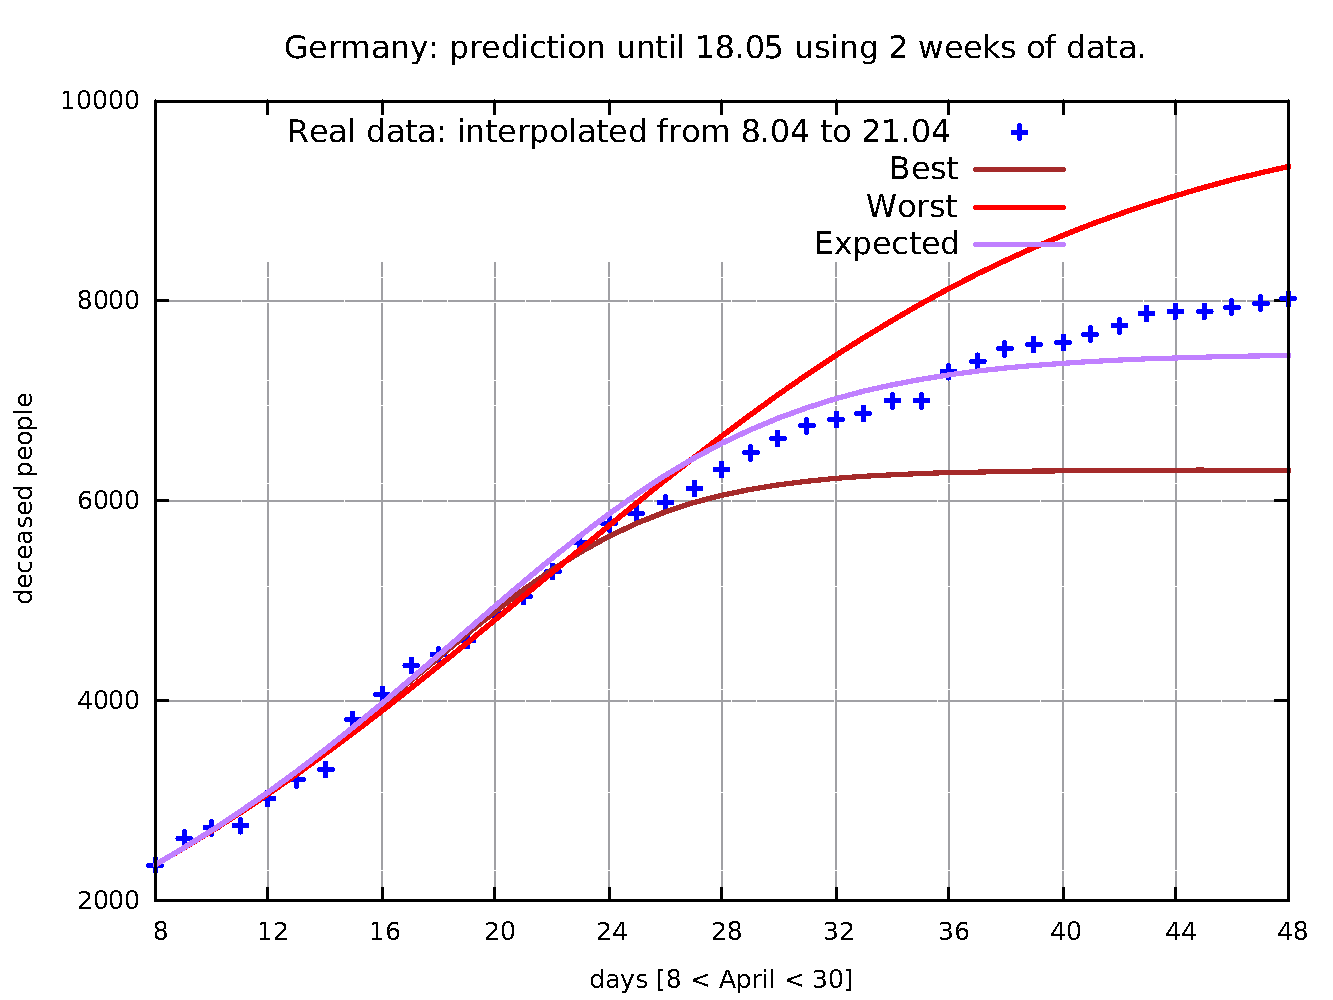
\includegraphics[width=\linewidth]{../simulations_v1/de/8-21/8-21.pdf}
  \end{subfigure}
  \begin{subfigure}[b]{0.45\linewidth}
  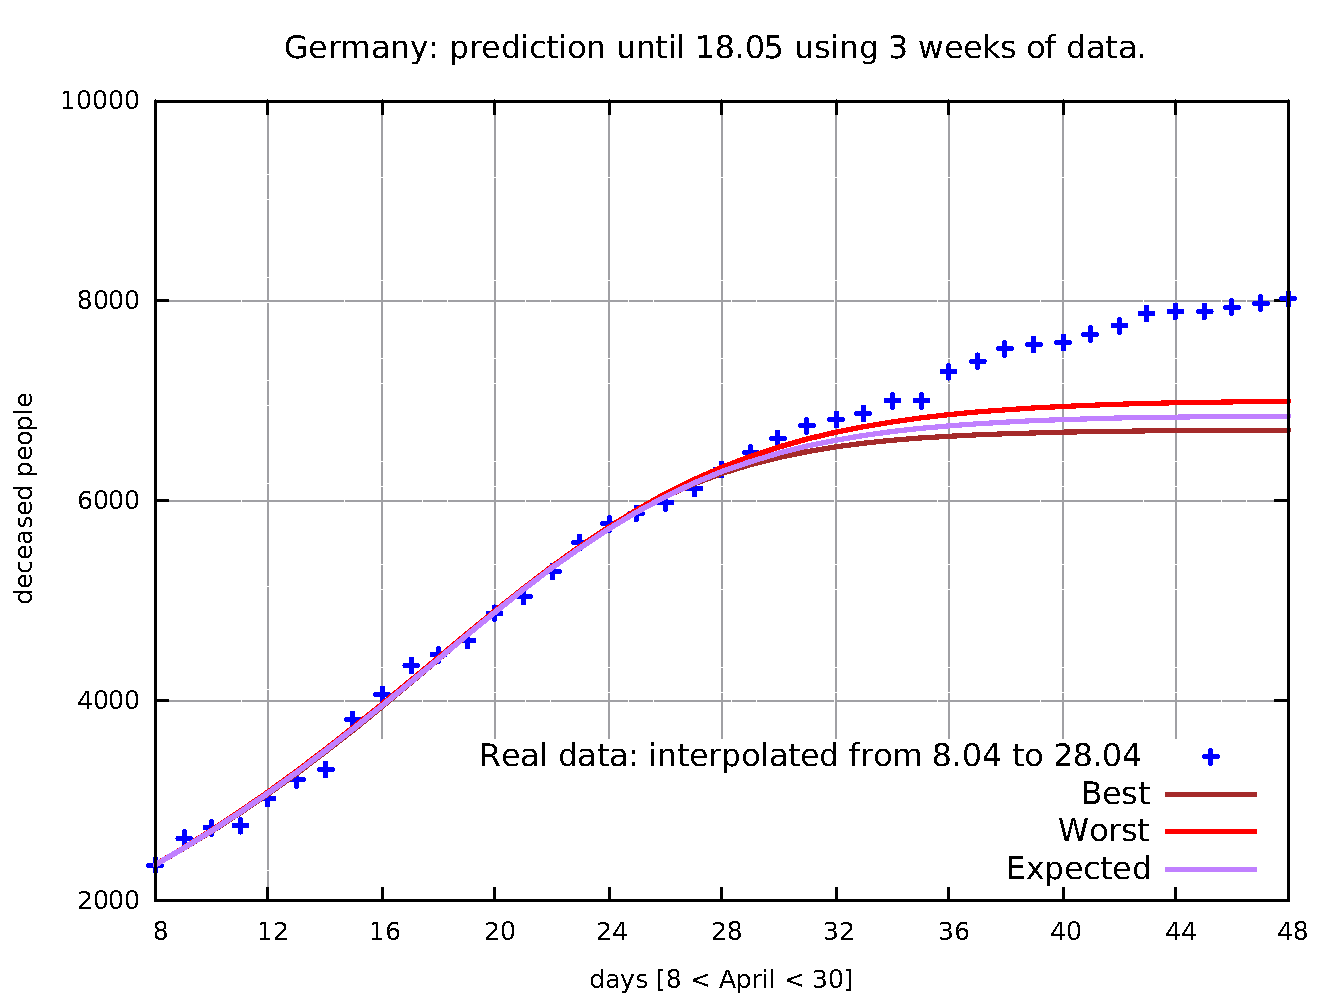
\includegraphics[width=\linewidth]{../simulations_v1/de/8-28/8-28.pdf}
  \end{subfigure}
	\caption{Germany -}
\end{figure}



\begin{figure}[h!]
  \centering
  \begin{subfigure}[b]{0.45\linewidth}
  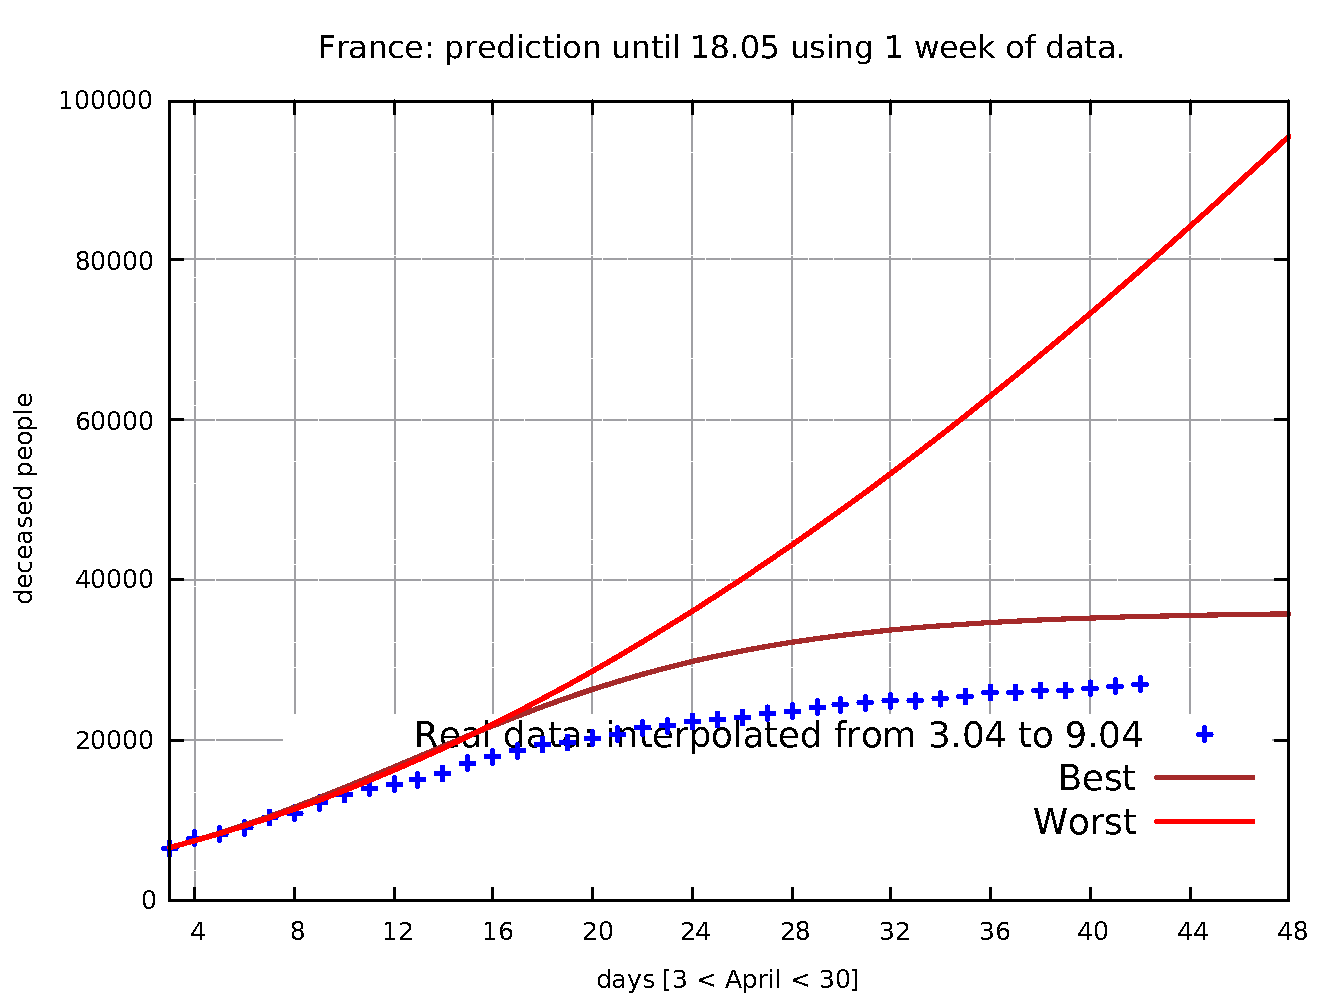
\includegraphics[width=\linewidth]{../simulations_v1/fr/3-9/3-9.pdf}
  \end{subfigure}
  \begin{subfigure}[b]{0.45\linewidth}
    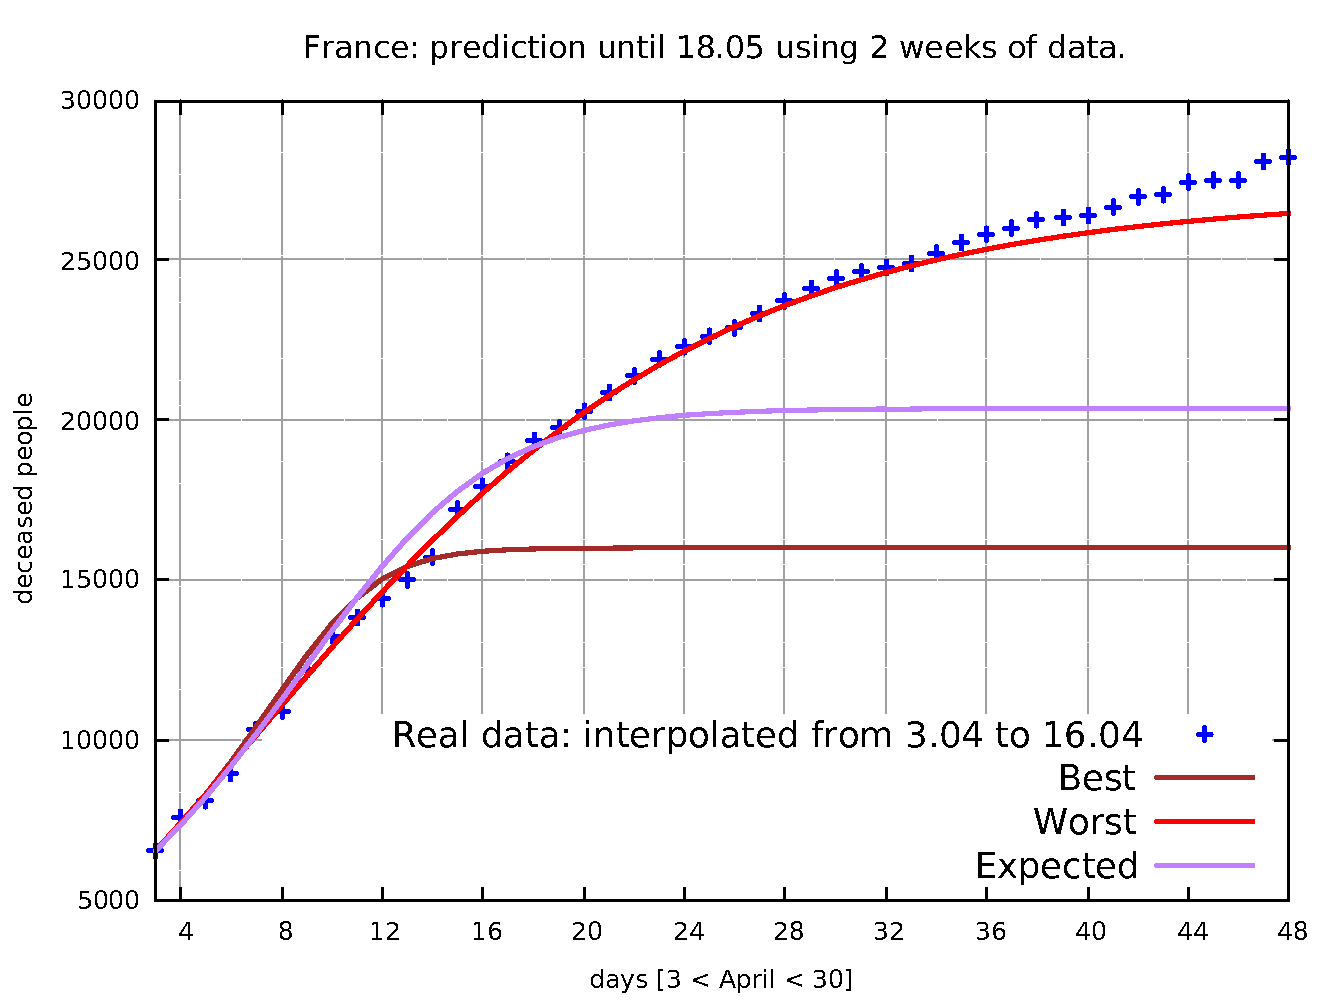
\includegraphics[width=\linewidth]{../simulations_v1/fr/3-16/3-16.pdf}
  \end{subfigure}
  \begin{subfigure}[b]{0.45\linewidth}
  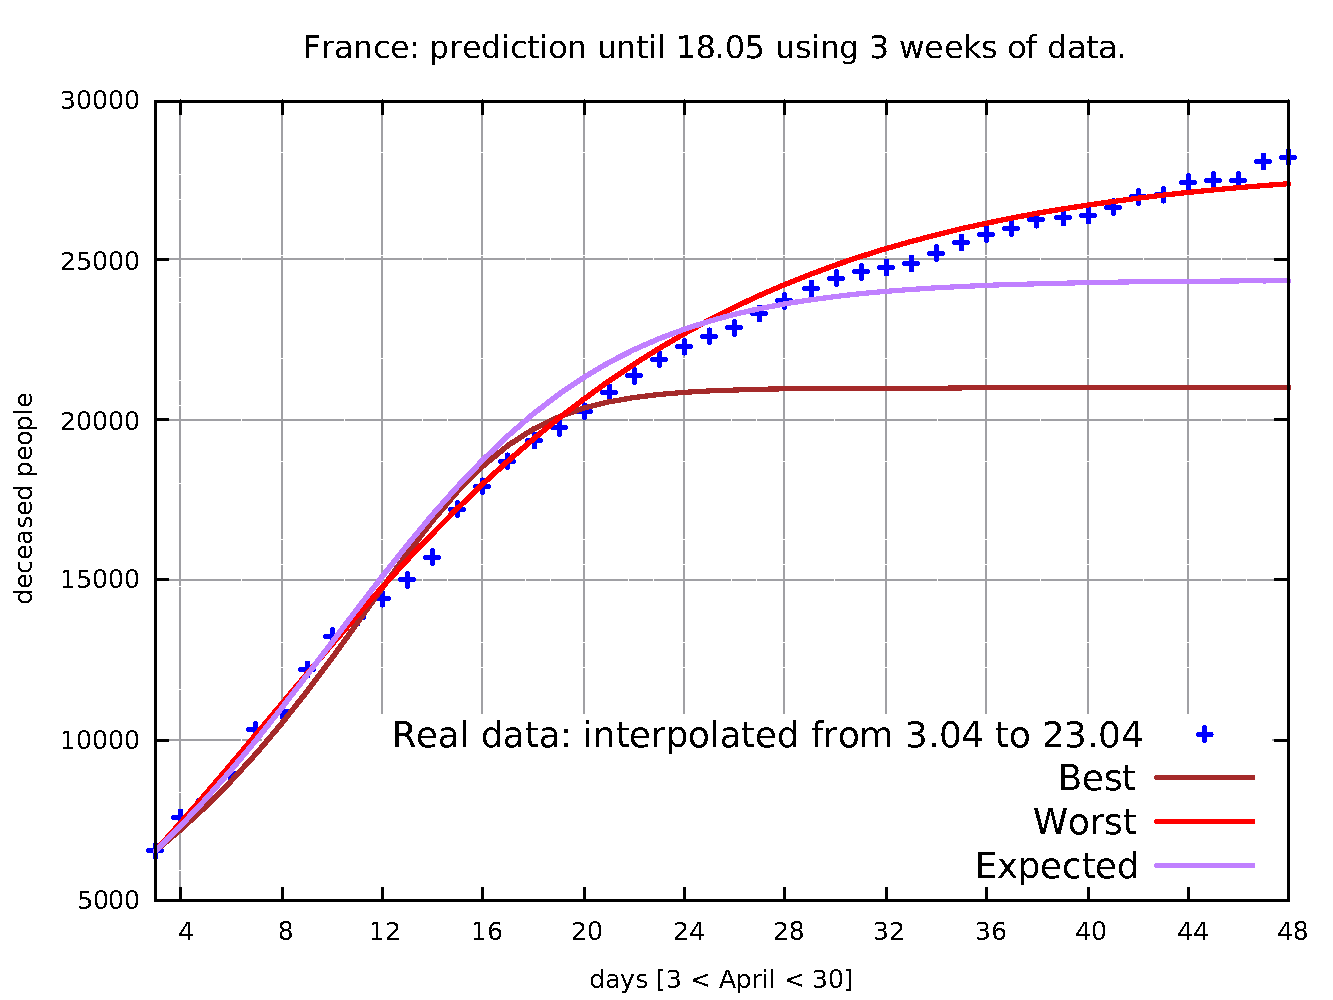
\includegraphics[width=\linewidth]{../simulations_v1/fr/3-23/3-23.pdf}
  \end{subfigure}
	\caption{France - to write}
\end{figure}


\begin{figure}[h!]
  \centering
  \begin{subfigure}[b]{0.45\linewidth}
  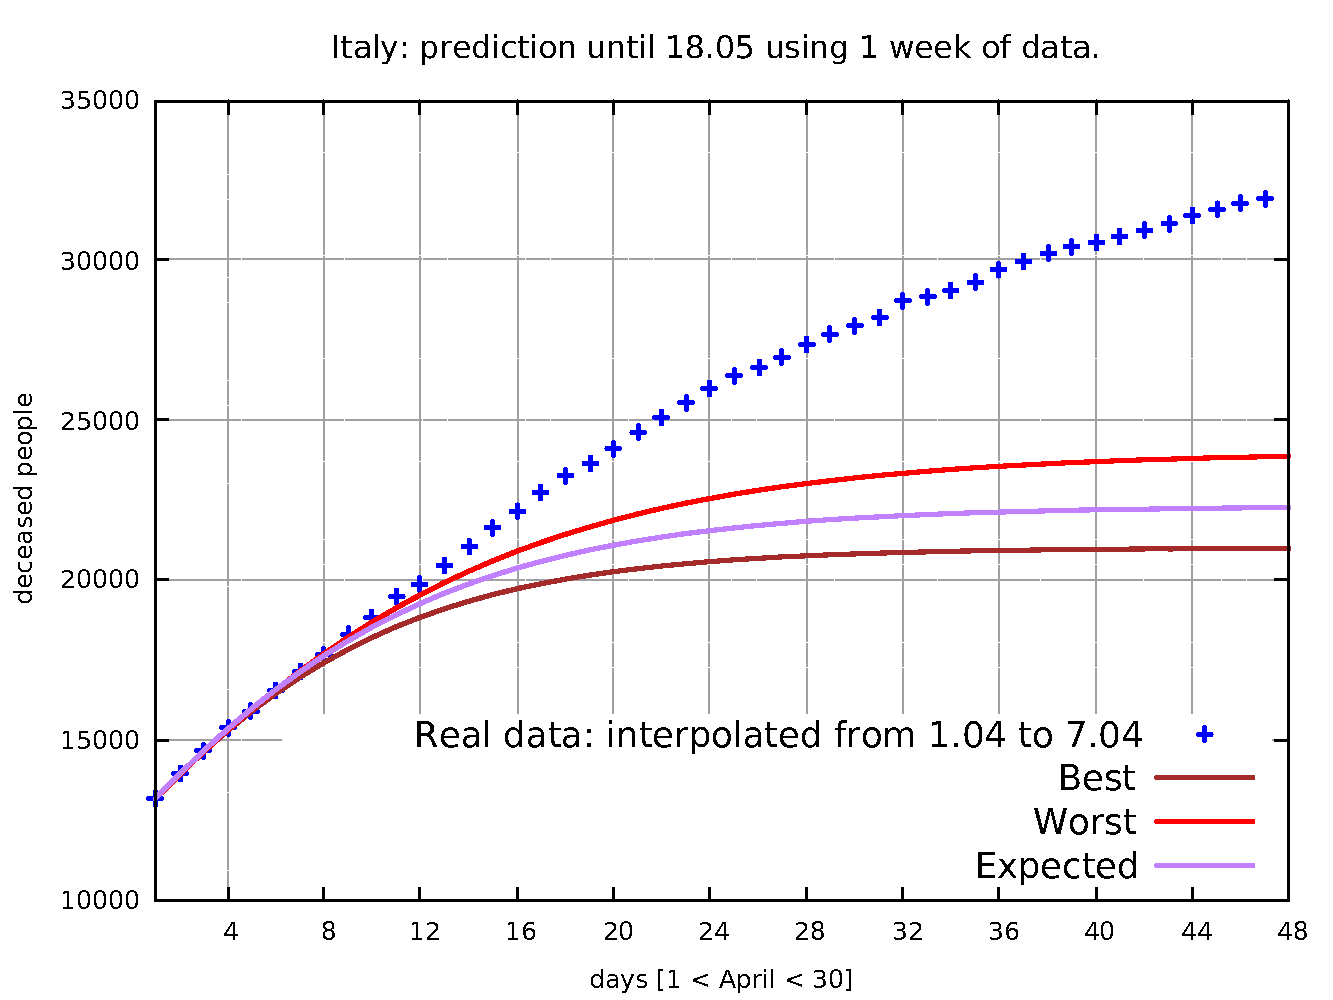
\includegraphics[width=\linewidth]{../simulations_v1/sp/1-7/1-7.pdf}
  \end{subfigure}
  \begin{subfigure}[b]{0.45\linewidth}
    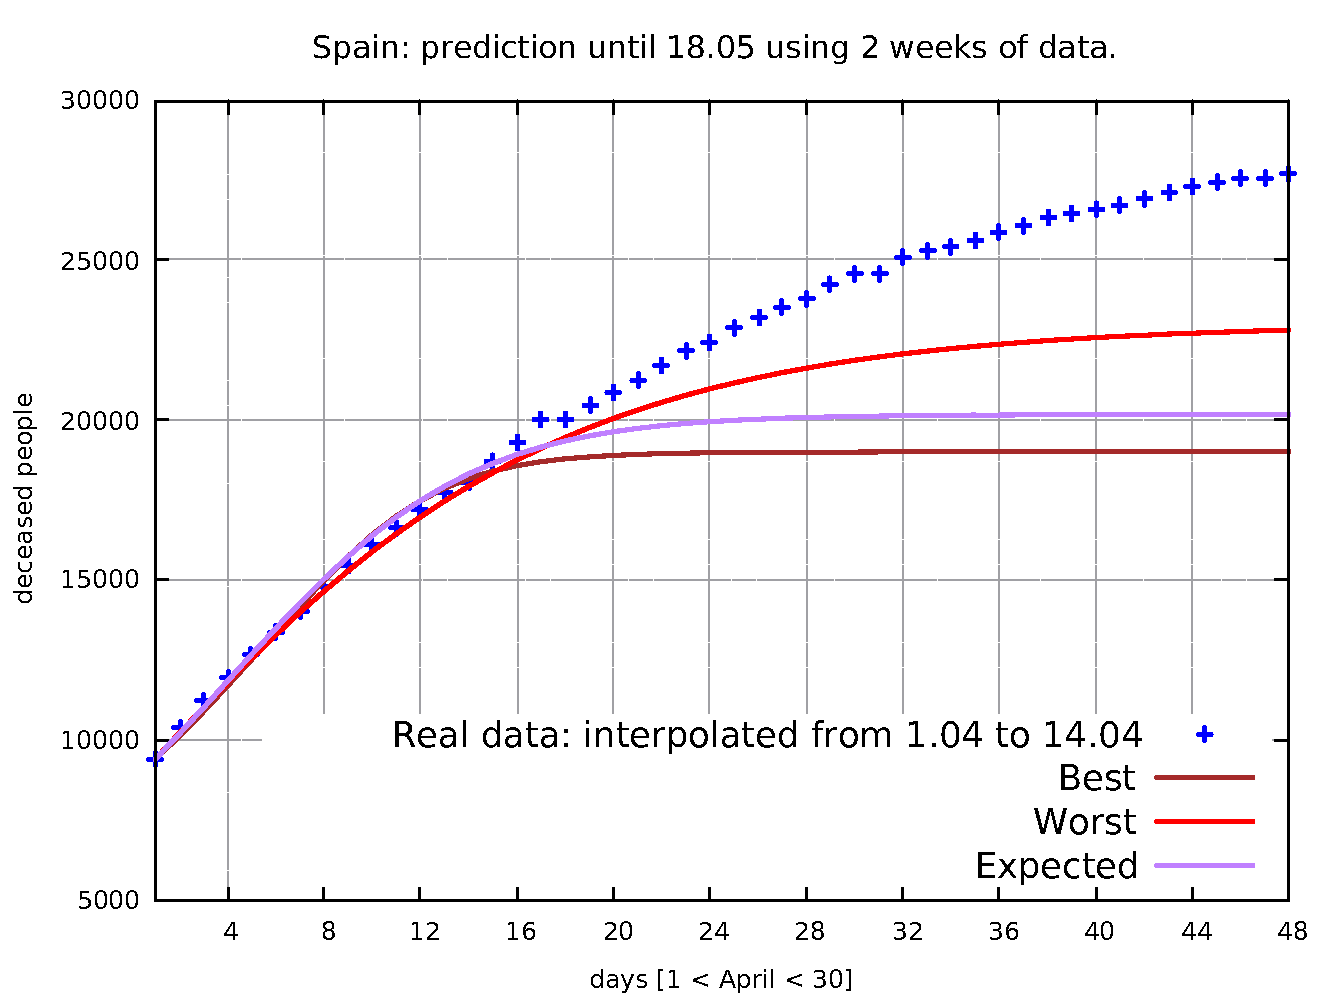
\includegraphics[width=\linewidth]{../simulations_v1/sp/1-14/1-14.pdf}
  \end{subfigure}
  \begin{subfigure}[b]{0.45\linewidth}
  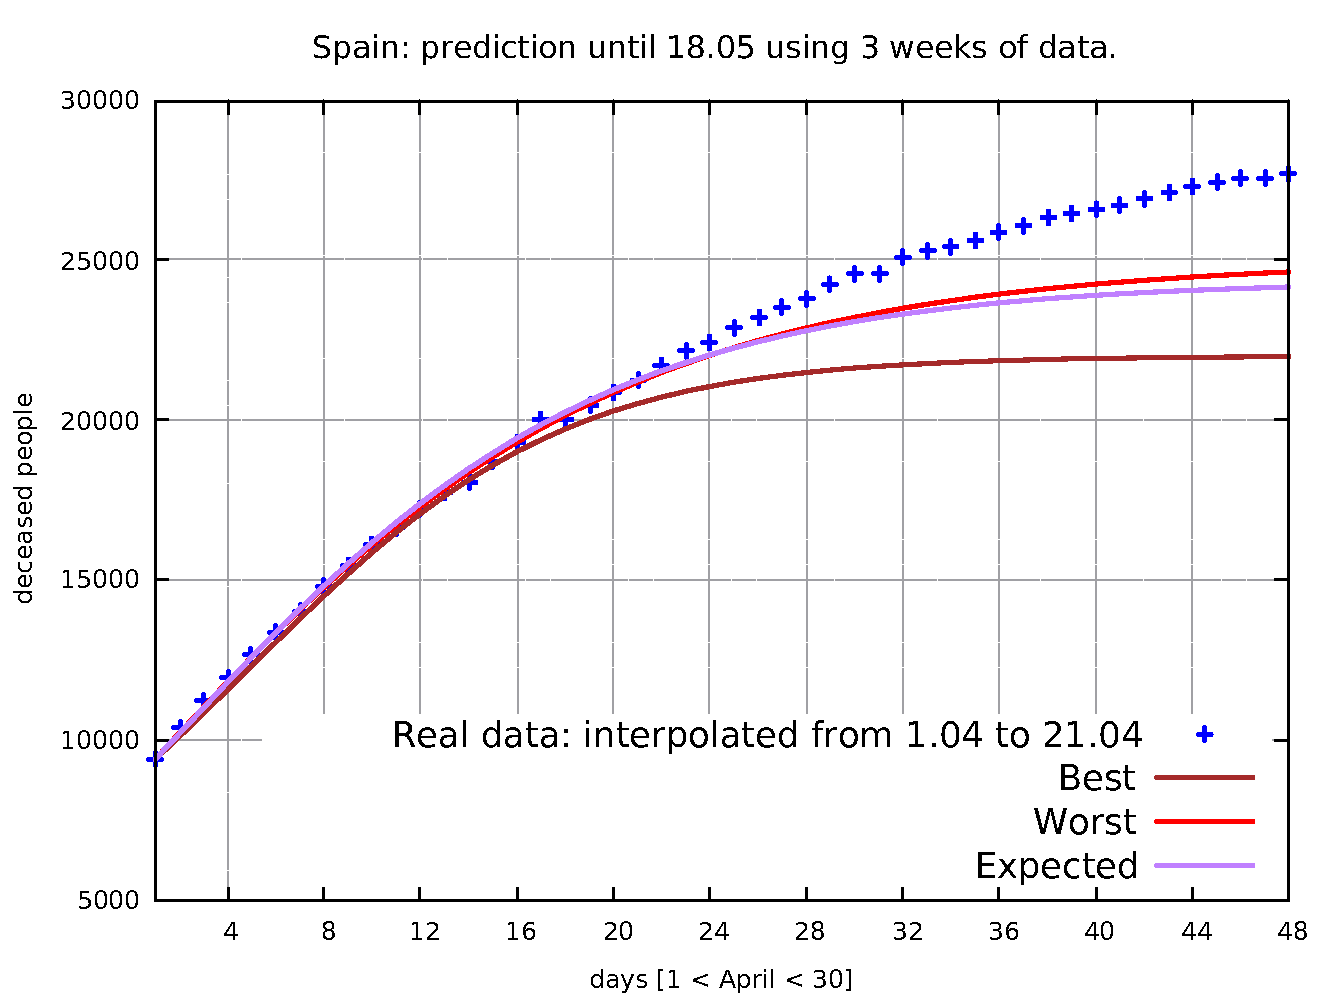
\includegraphics[width=\linewidth]{../simulations_v1/sp/1-21/1-21.pdf}
  \end{subfigure}
	\caption{Spain - to write}
\end{figure}


\begin{figure}[h!]
  \centering
  \begin{subfigure}[b]{0.45\linewidth}
  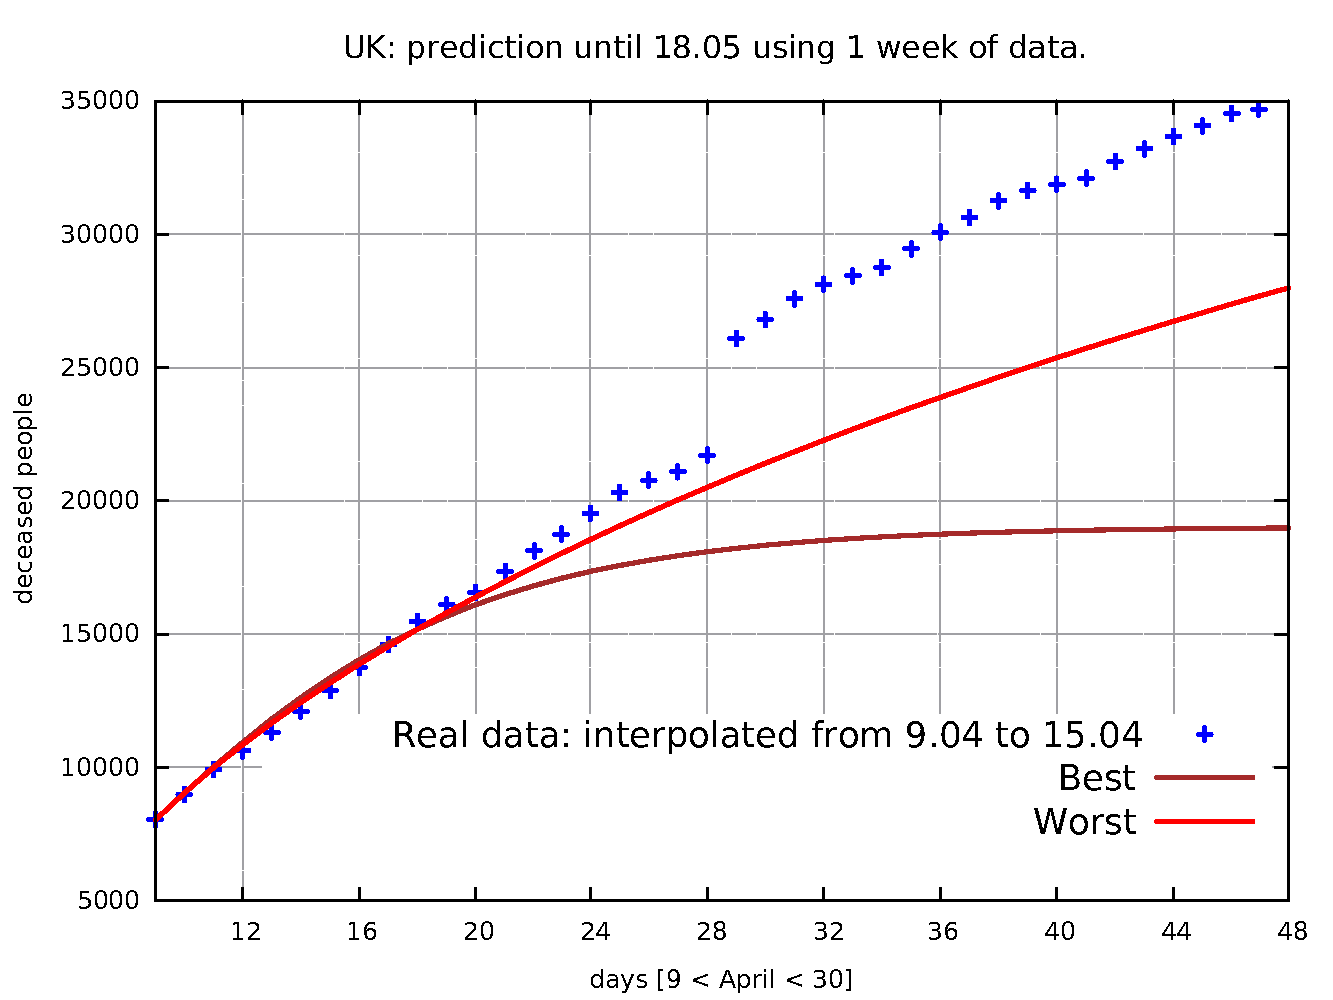
\includegraphics[width=\linewidth]{../simulations_v1/uk/9-15/9-15.pdf}
  \end{subfigure}
  \begin{subfigure}[b]{0.45\linewidth}
    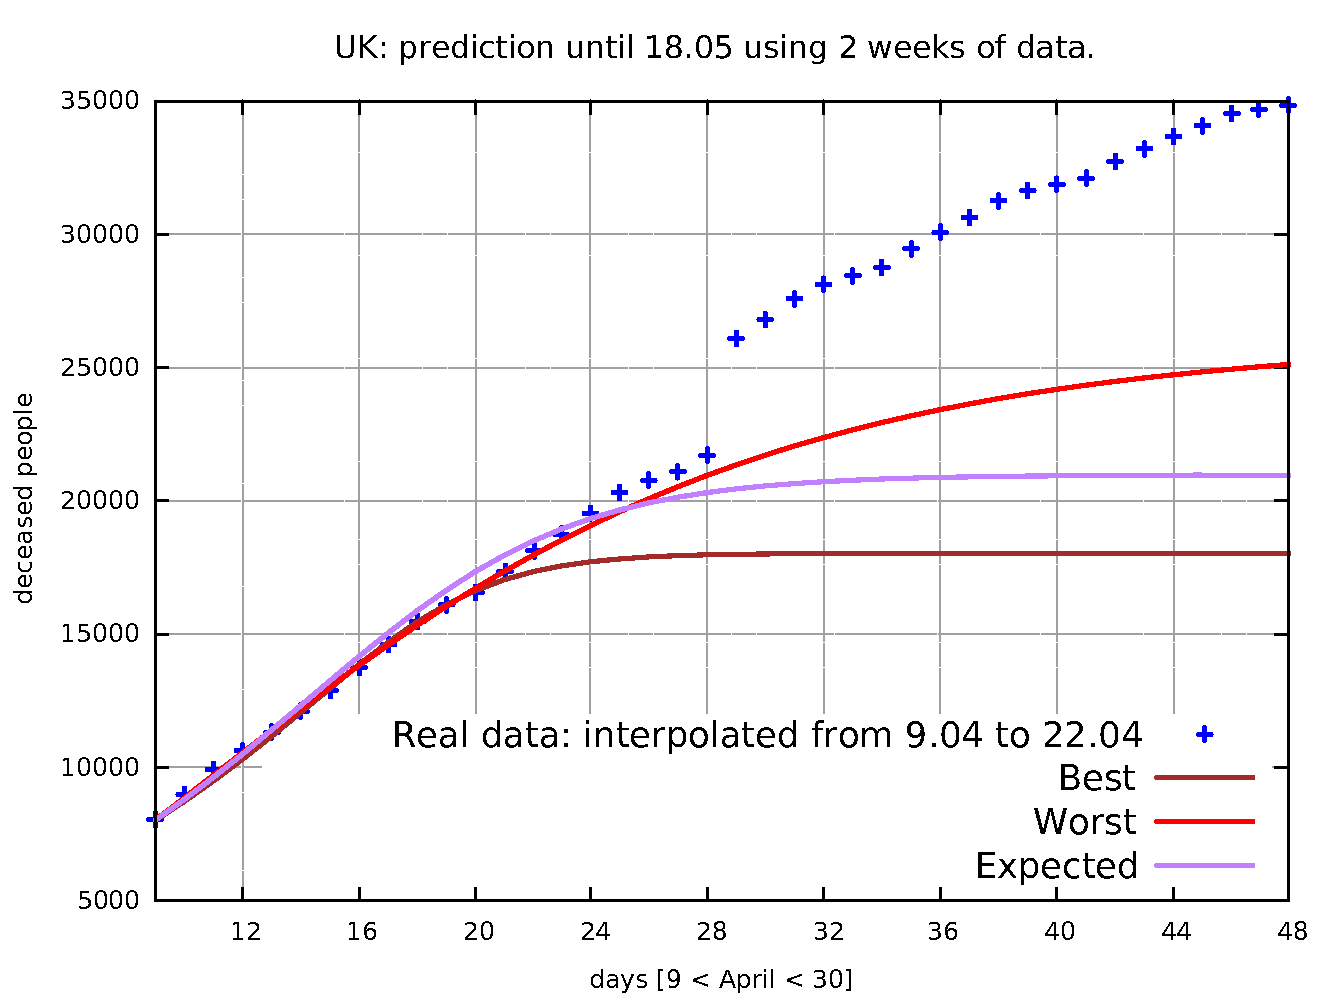
\includegraphics[width=\linewidth]{../simulations_v1/uk/9-22/9-22.pdf}
  \end{subfigure}
  \begin{subfigure}[b]{0.45\linewidth}
  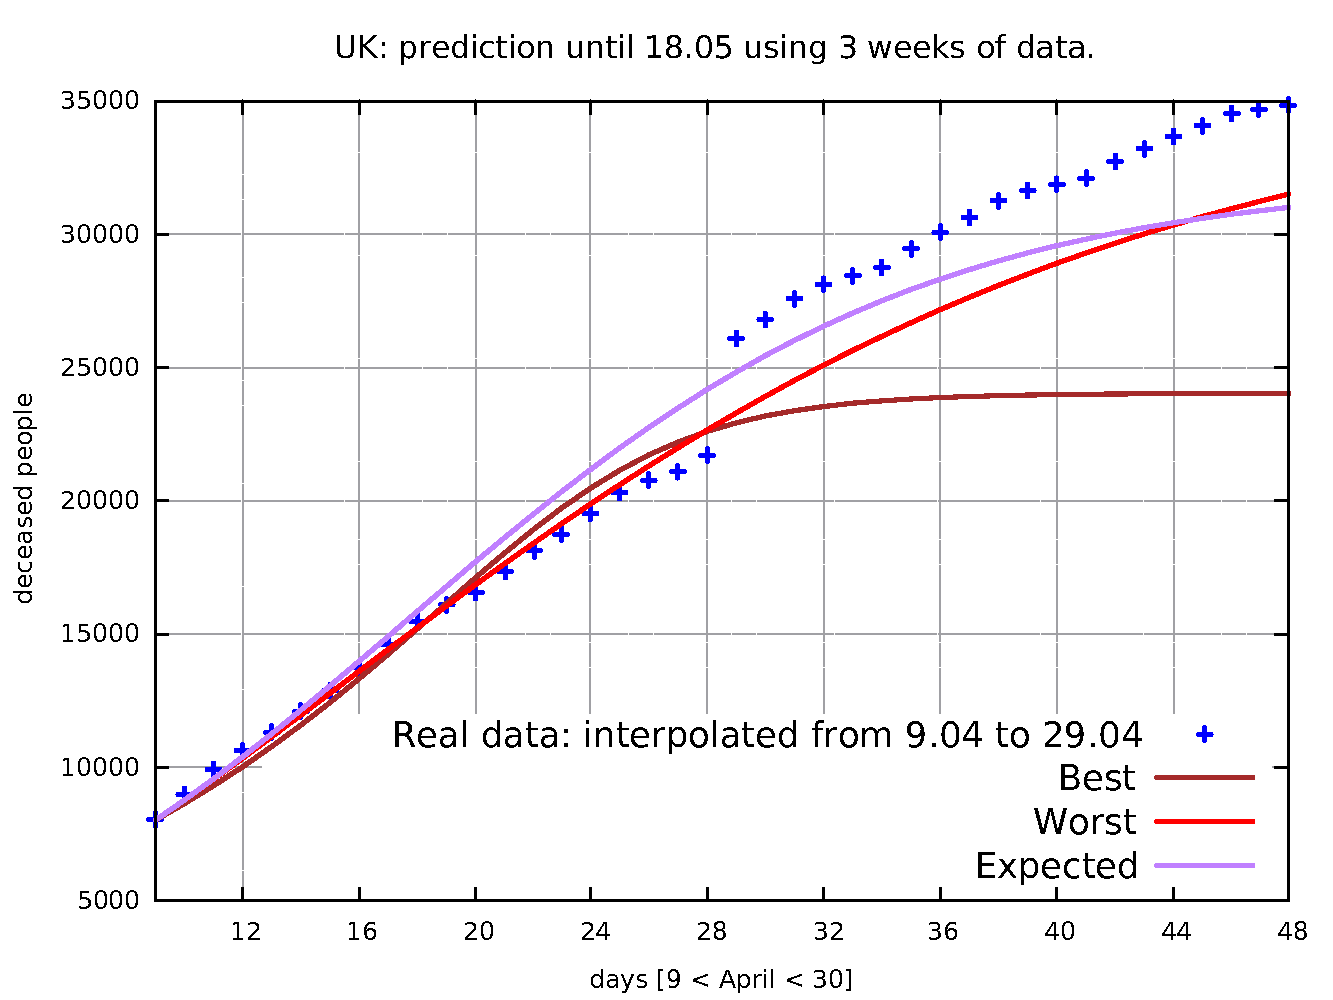
\includegraphics[width=\linewidth]{../simulations_v1/uk/9-29/9-29.pdf}
  \end{subfigure}
	\caption{UK - to write}
\end{figure}

\end{document}
